\documentclass[%
  a4paper,    
  parskip=half,
  twoside=true,
  %openright,      % start new chapters on an even-numbered page (right)
  draft=false,
]{scrreprt}

% **************************************** 
% Information
% **************************************** 
\newcommand{\thesisTitle}{Generierung angepasster RDF-Dumps von Wikidata}
\newcommand{\thesisName}{Benno Fünfstück}
\newcommand{\thesisSubject}{Bachelorarbeit}
\newcommand{\thesisDate}{Oktober 15, 2019}
\newcommand{\thesisVersion}{My First Draft}

\newcommand{\thesisFirstReviewer}{Prof. Markus Kroetzsch}
\newcommand{\thesisFirstReviewerUniversity}{\protect{Technische Universität Dresden}}
\newcommand{\thesisFirstReviewerDepartment}{Fakultät Informatik}

\newcommand{\thesisSecondReviewer}{Prof. Sebastian Rudolph}
\newcommand{\thesisSecondReviewerUniversity}{\protect{Technische Universität Dresden}}
\newcommand{\thesisSecondReviewerDepartment}{\protect{Fakultät Informatik}}

\newcommand{\thesisFirstSupervisor}{Prof. Markus Krötzsch}
\newcommand{\thesisSecondSupervisor}{Prof. Sebastian Rudolph}

\newcommand{\thesisUniversity}{\protect{Technische Universität Dresden}}
\newcommand{\thesisUniversityDepartment}{Fakultät Informatik}
\newcommand{\thesisUniversityInstitute}{Institut für Theoretische Informatik}
\newcommand{\thesisUniversityGroup}{Professur für Wissensbasierte Systeme}
\newcommand{\thesisUniversityCity}{}
\newcommand{\thesisUniversityStreetAddress}{01062 Dresden}
\newcommand{\thesisUniversityPostalCode}{}

% **************************************** 
% Load and Configure packages 
% **************************************** 

% setup german for XeLaTeX
\usepackage{polyglossia}
\setmainlanguage[spelling=new,babelshorthands=true]{german}
\usepackage{fontspec}

\PassOptionsToPackage{% setup clean thesis style
  figuresep=colon,%
  hangfigurecaption=false,%
  hangsection=true,%
  hangsubsection=true,%
  sansserif=false,%
  configurelistings=true,%
  colorize=full,%
  colortheme=bluemagenta,%
  configurebiblatex=true,%
  bibsys=biber,%
  bibfile=bib-refs,%
  bibstyle=alphabetic,%
  bibsorting=nty,%
}{cleanthesis}
\usepackage{cleanthesis}

\hypersetup{% setup the hyperref-package options
  pdftitle={\thesisTitle},    %   - title (PDF meta)
  pdfsubject={\thesisSubject},%   - subject (PDF meta)
  pdfauthor={\thesisName},    %   - author (PDF meta)
  plainpages=false,           %   -
  colorlinks=false,           %   - colorize links?
  pdfborder={0 0 0},          %   -
  breaklinks=true,            %   - allow line break inside links
  bookmarksnumbered=true,     %
  bookmarksopen=true          %
}

\usepackage{cleveref}
\usepackage{bookmark}

% avoid large space before paragraphs with title
\RedeclareSectionCommand[beforeskip=0pt]{paragraph}


\begin{document}

\frenchspacing

\pagenumbering{roman}			% roman page numbing (invisible for empty page style)
\pagestyle{empty}				% no header or footers
\input{content/titlepages}		% INCLUDE: all titlepages
\cleardoublepage

\pagestyle{plain}				% display just page numbers
% !TEX root = ../my-thesis.tex
%
\pdfbookmark[0]{Abstract}{Abstract}
\addchap*{Kurzfassung}
\label{sec:abstract}
Die freie Wissensdatenbank Wikidata bietet Exporte der Daten als RDF an.
Die Größe dieser Exporte stellt jedoch ein Hindernis für die Verarbeitung dar.
Auf Basis von Wikidata Toolkit wird in dieser Arbeit eine Anwendung entwickelt, die Dumps für Teile der Daten generiert.
Die Anwendung erlaubt es den Nutzern, eigene Kriterien zum Filtern der Exporte anzugeben.
Zur Überprüfung der Konsistenz dieser Dumps mit den vollständigen Exporten wird ein Vergleich durchgeführt.
Dabei wird das von Wikidata Toolkit erzeugte RDF mit den Wikidata-Exporten verglichen.
Mit dieser Methode werden mehrere Fehler in Wikidata Toolkit aufgedeckt.
Durch Beheben dieser Fehler leistet die Arbeit einen Beitrag zur Verbesserung des RDF-Exports von Wikidata Toolkit.
Mit der entwickelten Anwendung wird die Verwendung von Daten aus Wikidata vereinfacht.

\vspace*{20mm}

{\usekomafont{chapter}Abstract}
\label{sec:abstract-diff}

Wikidata, a free knowledge base, provides data exports in RDF.
However, usage of these exports is a challenge due to their large size.
In this work we present an application based on Wikidata-Toolkit that solves this problem by providing dumps of parts of the data.
User-defined criteria allow fine-grained filtering of the exports.
To verify the consistency of dumps generated this way, we perform a comparision.
In this comparision, RDF as generated by Wikidata-Toolkit is compared to the full RDF exports provided by Wikidata.
Multiple issues in Wikidata-Toolkit are uncovered.
In addition to developing a useful tool for consumers of Wikidata exports, we contribute several fixes to Wikidata-Toolkit.		% INCLUDE: the abstracts (english and german)
\cleardoublepage
%
%\input{content/acknowledgement} % INCLUDE: acknowledgement
%\cleardoublepage
%
\currentpdfbookmark{\contentsname}{toc}
\setcounter{tocdepth}{2}		% define depth of toc
\tableofcontents				% display table of contents
\cleardoublepage

% --------------------------
% Body matter
% --------------------------
\pagenumbering{arabic}			% arabic page numbering
\setcounter{page}{1}			% set page counter
\pagestyle{scrheadings}			% header and footer style

\typeout{CONTENT START NOW}
% !TEX root = ../thesis.tex
%
\chapter{Einleitung}
\label{sec:intro}

  
% !TEX root = ../thesis.tex
%
\chapter{Hintergrund}
\label{sec:concepts}

\section{Wikidata}
\cite{wikidata}

\subsection{Wissensgraphen}
\subsection{Datenmodell}

\section{RDF}
\cite{rdf-dump-format}
      
\chapter{Anforderungen}
\label{chap:requirements}

\section{funktionale Anforderungen}
Im Fokus dieser Arbeit steht die Entwicklung eines Systems zur Filterung des RDF-Exports von Wikidata.
Damit sollen Wissenschaftler mit wenig Aufwand Dumps nach speziellen Kriterien erstellen können.
Die wesentlichen Merkmale des Systems sind:

\begin{description}
  \item[Format] Der Dump soll als RDF im N-Triples Format erstellt werden. Damit die gefilterten Dumps möglichst kompatibel mit dem vollständigen Wikidata RDF Dump sind, sollte das Schema dem offiziellen RDF-Dump-Format entsprechen. Erweiterungen des Schemas müssen klar gekennzeichnet sein.
  \item[Filterung] Nutzer sollen über eine einfache Oberfläche wählen können, welche Entitäten in welchem Detailgrad im erstellten Dump enthalten sind. 
  \item[Archivierung] Damit die Dumps in wissenschaftlichen Veröffentlichungen zitiert werden können, muss die Verfügbarkeit auch in ferner Zukunft garantiert werden. Deshalb ist eine Methode zur Langzeitarchivierung generierter Dumps notwendig. 
  \item[Suche] es soll eine durchsuchbare Übersicht über alle erstellen Dumps.
    So können Ideen anderer Nutzer als Vorlage dienen und nicht jeder Nutzer muss sich eigene Filterregeln ausdenken,
  \item[Statistiken] Um schnell zu entscheiden, ob ein Dump für einen bestimmten Anwendungsfall geeignet ist, sollten Statistiken über den Inhalt (z.B. die Anzahl der Entitäten) des Dumps angezeigt werden. Zusätzlich sollten auch schon während der Generierung Statistiken zum Fortschritt des Dumps bereitgestellt werden.
  \item[Nachvollziehbarkeit] Gerade für den wissenschaftlichen Einsatz ist es erforderlich, dass die Herkunft der Daten und Generierung nachvollziehbar ist. Es sollte demnach leicht sichtbar sein, wie der Dump entstanden ist und eine Reproduktion des Dumps mit diesen Daten möglich sein. 
  \item[Aktualität der Daten] Die Dumps sollten aus möglichst aktuellen Daten erstellt werden.
    Es ist natürlich nicht notwendig, dass die Dumps immer komplett aktuell sind, aber die Daten zur Generierung der Dumps sollten regelmäßig aktualisiert werden.
\end{description}

\section{nicht-funktionale Anforderungen}
Neben den Anforderungen an die Funktion des Systems existieren auch eine Reihe von weiteren Anforderungen:

\begin{description}
  \item[Hardwareanforderungen] Der Ressourcenverbrauch des Systems sollte in einem akzeptablen Rahmen liegen.
  Als Anhaltspunkte für die Beurteilung dienen hier vergleichbare Systeme, wie bspw. der Wikidata Query Service, welcher ebenfalls Services basierend auf den RDF-Daten von Wikidata anbietet und gleichzeitig deutlich populärer ist. Demnach sollte das System entsprechend seiner Relevanz geringere Hardwareanforderungen als der Wikidata Query Service haben.
\item[Freie Lizenz] Die Wikimedia Foundation legt großen Wert darauf, möglichst viele der verwendeten Tools unter einer freien Lizenz bereitzustellen\cite{wikimedia-guiding-principles}.
  Wenn das System in der Wikimedia Cloud betrieben werden soll, dann ist die Veröffentlichung des Quellcodes unter einer freien Lizenz sogar Pflicht\cite{wikimedia-cloud-tos}.
\item[Bearbeitungszeit] Das System sollte maximal einen Tag zur Generierung eines Dumps benötigen, besser unter 12 Stunden. Während längerer Prozesse sollte keine ständig Verfügbarkeit des Nutzers erwartet werden. 
\item[Erweiterbarkeit] Da die funktionalen Anforderungen an das System sehr allgemein sind, muss auf Erweiterbarkeit geachtet werden sodass neue Anforderungen einfach umgesetzt werden können. Es sind beispielsweise viele verschiedene Filtermöglichkeiten und Statistiken denkbar, die nicht alle in der ersten Version umgesetzt werden können. Es ist daher sinnvoll vor allem in diesem Bereich auf Erweiterbarkeit zu achten.
\item[Skalierbarkeit] Wikidata wächst beständig, aktuell existieren etwas weniger als 59 Millionen Items.\TODO{cite}
  Insgesamt gibt es über 700 Millionen Statements und diese Zahl ist allein im letzten Jahr um 200 Millionen gewachsen. Das System muss also mit dieser Menge an Daten umgehen können und dies auch für die nächsten Jahre noch leisten können.
\end{description}

\section{Verwandte Arbeiten}
Zu den verwandten Projekten gehört sicherlich der Wikidata Query Service\cite{wd-sparql}, welcher bereits einen gezielten Zugriff auf die Daten gewährt.
Die Daten des Query Services entsprechen bis auf wenige Minuten Verzögerung der neusten Wikidata Version.
Da der Query Service allerdings beliebige SPARQL-Abfragen erlaubt, ist ein Timeout von einer Minute notwendig um zu großen Ressourcenverbrauch abzufangen, denn bei SPARQL-Abfragen kann die Termination nicht sichergestellt werden.
Für die Erzeugung von großen Dumps ist der Query Service damit ungeeignet.

Zwei weitere existierende APIs, der Linked Data Export von Wikidata und die Wikidata API, skalieren ebenso nicht für größere Abfragen.
Mit dem Linked Data Export können die RDF und JSON Daten einzelner Items über HTTP abgerufen werden.
Die API erlaubt das Abrufen der JSON Daten von bis zu 50 Items in einer Anfrage.
Beide Varianten sind daher nur für den Abruf einer kleinen Menge an Items geeignet.

Ein Mittelweg zwischen Abfragekomplexität für den Server und Anzahl an Abfragen an der Server beschreibt die Linked Data Fragments\cite{ldf} Spezifikation.
Allerdings führt dies zu hohen Abfragekosten auf dem Client, da die Joins auf dem Client ausgewertet werden.
Die Implementierung für Wikidata basiert außerdem auf der selben RDF-Datenbank wie auch der Wikidata Query Service.
Im Kontext von Wikidata haben Linked Data Fragments daher keinen Vorteil gegenüber dem Query Service.

Eine Variante zur Reduzierung der Größe von RDF-Dumps ist HDT\cite{hdt}, einem Binärformat für RDF-Daten.
Es verwendet eine optimierte, komprimierte Kodierung zur Speicherung der Dumps.
Auf diesem Format lassen sich sogar einfache SPARQL-Abfragen effizient ausführen\cite{hdt-query}.
Leider erfordert die Erstellung von HDT-Dumps viel Arbeitsspeicher und Rechenzeit, besonders bei einer so großen Datenmenge wie Wikidata.
Durch die komprimierte Kodierung ist eine inkrementelle Aktualisierung von HDT-Dumps nicht möglich, sodass der komplette Dump regelmäßig neu erstellt werden müsste.

DBpedia\cite{dbpedia} teilt die seine Dumps in mehrere, kleinere Dumps auf.
Auch einige aus Wikidata abgeleitete Dumps sind verfügbar\footnote{\url{https://databus.dbpedia.org/dbpedia/wikidata/}}.
Durch das fest definierte Schema ist eine solche Trennung der Datensätze bei DBpedia möglich.
Für Wikidata ist dieser Ansatz deutlich schwieriger, da das Datenschema so flexibel ist.
Es gibt in Wikidata damit einzelnen Aspekt, nach dem diese Trennung erfolgen könnte.

Ein mächtiges Tool zum Erstellen von Listen von Wikidata Items ist PetScan\footnote{\url{https://petscan.wmflabs.org/}}.
Dieses Tool bietet ein User-Interface mit einer Vielzahl an Optionen, um Listen von Wikipedia bzw. Wikidata-Seiten zu erstellen.
Wikidata ist nicht der Hauptanwendungszweck dieses Tools, dennoch ist es eine interessante Quelle von Filtern.  
\chapter{Design}

\section{Architektur}
client only, dump processor (RDF vs JSON dumps), indexing, sparql based

\section{Auswahl externer Dienste}
Archivierung: Vergleich Anbieter (Zenodo)
Hosting: auf toolforge

\section{Interface}        
\chapter{Implementierung}
\label{chap:implementation}
Die Anwendung besteht aus zwei Teilen: Backend und Frontend.
Der Hauptteil der Anwendung läuft auf einem Server.
Das Frontend hat eine JavaScript-Komponente für das User-Interface, welche auf dem Client ausgeführt wird.
Über das Frontend können Nutzer Aufträge für Dumps erstellen und existierende Dumps verwalten, während das Backend nur für die Generierung von Dumps zuständig ist.

Das Design der Anwendung verwendet eine Warteschlange zur Kommunikation zwischen Frontend und Backend.
Für die Implementierung wird diese Warteschlange über eine gemeinsame Datenbank realisiert, die bereits vom Frontend zur Verwaltung der Metadaten der Dumps eingesetzt wird.
In diesen Kapitel wird erst das Datenmodell vorgestellt, welches zur Kommunikation verwendet wird.
Danach wird die Implementierung von jeweils Frontend und Backend genauer beschrieben.

\section{Datenmodell}
\begin{figure}
  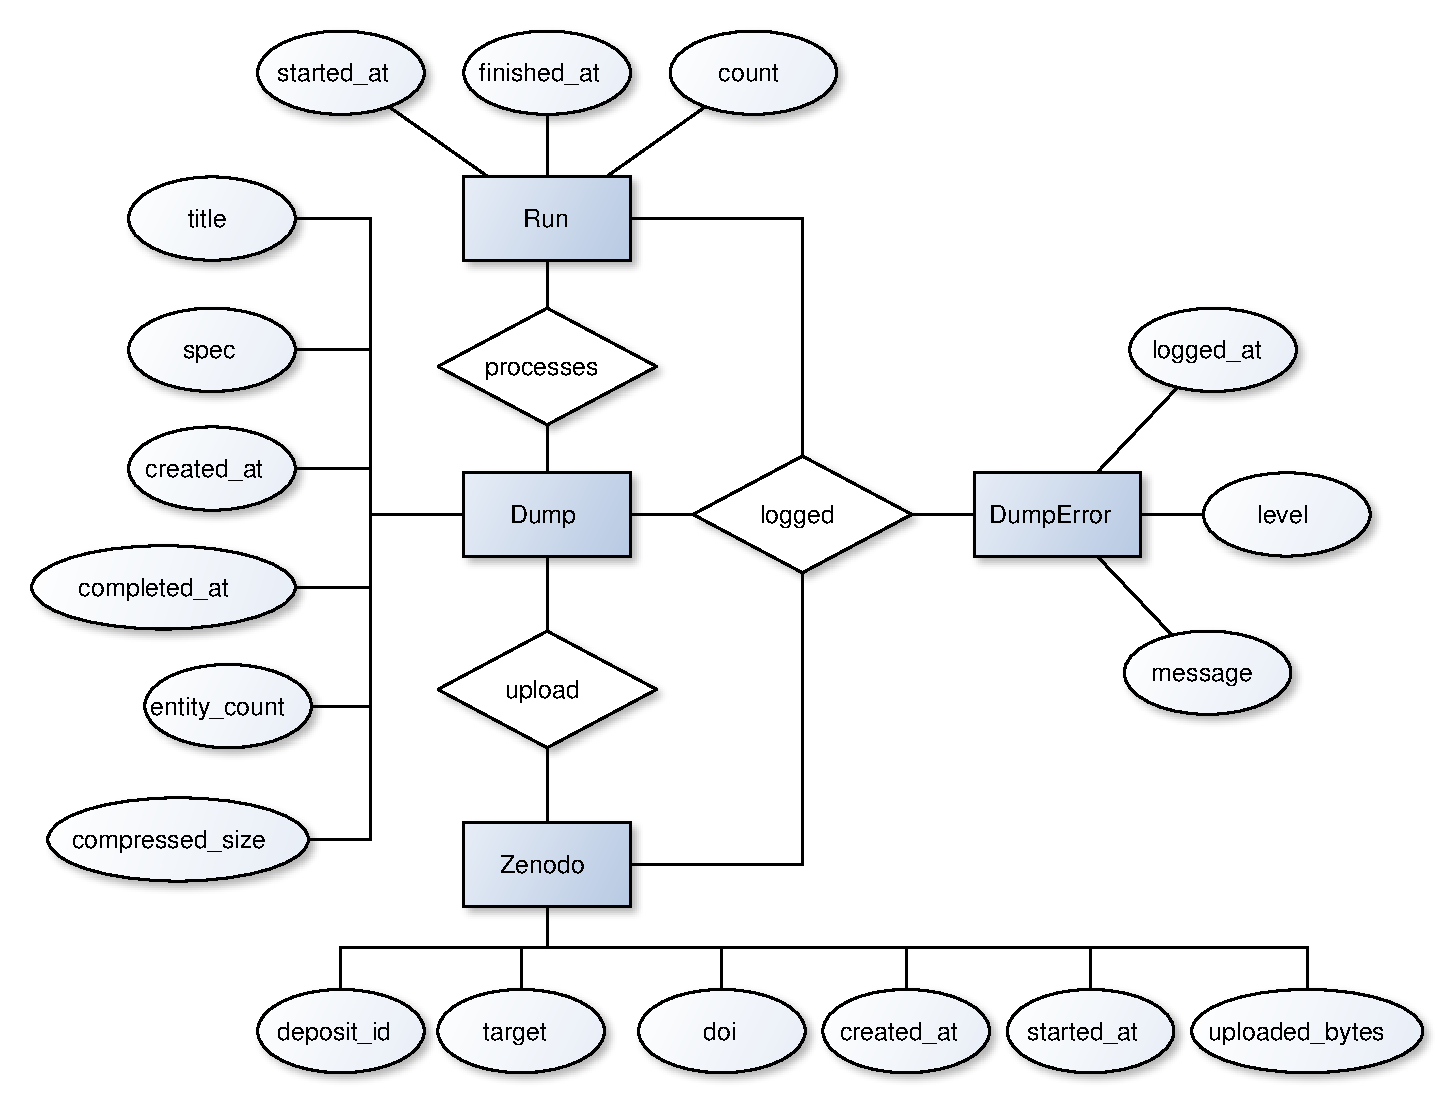
\includegraphics[width=\textwidth]{pics/db-er}
  \caption{Datenbankschema}
  \label{fig:db-er}
\end{figure}
Eine Übersicht des Datenmodells liefert \cref{fig:db-er}.
Das zentrale Element ist der Dump, welcher alle Metadaten zu einem Auftrag speichert.
Neben ein paar einfachen Daten wie Titel (\verb|title|) und Zeitpunkt der Erstellung des Auftrags (\verb|created_at|) bzw. Fertigstellung (\verb|completed_at|) ist jeder Dump durch eine JSON-Spezifikation (\verb|spec|) charakterisiert. Zusätzlich hat der Dump auch Felder für Statistiken, wie die Anzahl der Entitäten (\verb|entity_count|) und Dateigröße (\verb|compressed_size|).

Für jeden Durchlauf des Backends wird ein \verb|Run| angelegt.
Die von diesem Durchlauf verarbeiteten Aufträge verweisen dann auf den \verb|Run|.
Damit der aktuelle Fortschritt ermittelt werden kann, wird die Anzahl der bereits verarbeiteten Entities in dem Attribut \verb|count| gespeichert.
Die ungefähre Anzahl der Entitäten in dem vollen Wikidata-Dump ist aus vorherigen Durchläufen bekannt oder kann über den Wikidata Query Service mit einer Abfrage ermittelt werden.
Zusammen mit der Anzahl an bereits verarbeiteten Entities lässt sich daraus der Fortschritt errechnen.
Die \verb|started_at| und \verb|finished_at| Attribute speichern Start- und Endzeitpunkt des \verb|Run|s.
Für noch nicht abgeschlossene \verb|Run|s hat \verb|finished_at| den Wert \verb|NULL|.

In der Tabelle \verb|Zenodo| werden Uploads von Dumps verwaltet.
Für Uploads muss bei Zenodo ein Deposit angelegt werden.
Den Bezeichner dieses Deposits speichert \verb|deposit_id|.
Mit \verb|target| (\verb|RELEASE| oder \verb|SANDBOX|) wird die Zenodo-Instanz angegeben.
\verb|RELEASE| bezeichnet die Hauptinstanz, während \verb|SANDBOX| eine Instanz zum Testen ist.
Der von Zenodo generierte Digital Object Identifier wird in dem Attribut \verb|doi| gespeichert.
Zur Verwaltung und Anzeige des Fortschritts werden Zeitdaten (\verb|created_at| und \verb|started_at|) und die Anzahl der bis jetzt hochgeladenen Bytes gespeichert (\verb|uploaded_bytes|). 

Für Fehlermeldungen bei der Verarbeitung gibt es die Tabelle \verb|DumpError|. 
Fehlermeldungen können mit einem bestimmten \verb|Run|, \verb|Dump| und \verb|Zenodo| (Upload) verknüpft werden.
Jeder Fehler hat ein \verb|level| (\verb|CRITICAL|, \verb|WARNING|, \ldots), einen Zeitstempel (\verb|logged_at|) und eine Meldung (\verb|message|).

\section{Backend}
Für die Implementierung des Backends wird das Wikidata Toolkit\footnote{\url{https://github.com/Wikidata/Wikidata Toolkit}} verwendet.
Da Wikidata Toolkit in Java geschrieben ist, muss deswegen auch eine Java-kompatible Programmiersprache verwendet werden.
An dieser Stelle wurde Java gewählt, um auch die Wartbarkeit der Anwendung in Zukunft sicherzustellen, da Java im Vergleich zu anderen Programmiersprachen mit Java-Kompatibilität (wie zum Beispiel Scala\footnote{https://www.scala-lang.org/} oder Kotlin\footnote{\url{https://kotlinlang.org/}}) deutlich weiter verbreitet und bekannter ist.

Die Hauptschleife des Backends besteht aus zwei Phasen: Warten und Verarbeitung.
Während der wartenden Phase wird kontinuierlich auf neue Aufträge gewartet.
Sobald neue Aufträge verfügbar sind, wird die Verarbeitung gestartet. 
Neue Aufträge werden dann erst wieder nach Beendigung des aktuellen Verarbeitungsprozesses abgerufen.

Am Start befindet sich das Backend in der wartenden Phase.
Um neue Aufträge abzurufen, werden dazu periodisch die in \cref{lst:backend-waiting} dargestellten SQL-Befehle in einer Transaktion ausgeführt.
Da in Zeile 6 nur Aufträge zugewiesen werden, die noch keinem \verb|Run| zugewiesen sind, kann diese Abfrage theoretisch auch von mehreren Prozessen gleichzeitg ausgeführt werden ohne dabei Kollisionen zu erzeugen.
Es ist so unmöglich, dass ein Auftrag mehr als einem \verb|Run| zugwiesen wird, was die Robustheit des Systems erhöht.
Falls diese Befehle keine Ergebnisse liefern (wenn keine neuen Aufträge vorliegen), wird eine definierte Zeit gewartet bevor dieser Vorgang wiederholt wird.
Diese Wartezeit führt gleichzeitig dazu, dass mehrere Aufträge gesammelt werden können, da die Verarbeitung nicht direkt beginnt.

\begin{lstlisting}[language=SQL, caption={Abrufen neuer Aufträge}, label={lst:backend-waiting}]
-- neuen Run erstellen
INSERT INTO run () VALUES ()
-- generated id: 1

-- Aufträge dem Run zuweisen
UPDATE dump SET run_id = 1 WHERE run_id IS NULL

-- Zugewiesene Aufträge abrufen
SELECT id, spec FROM dump WHERE run_id = :run
\end{lstlisting}

Zum Verarbeiten der Aufträge wurde der in Wikidata Toolkit bereits vorhandene RDF-Export angepasst.
Der RDF-Export ist dabei als eine Klasse implementiert, welche das von Wikidata Toolkit erwartete Interface \verb|EntityDocumentProcessor| implementiert (\cref{lst:wd-processor-interface}).

\begin{lstlisting}[language=Java, caption={EntityDocumentProcessor Interface}, label={lst:wd-processor-interface}]
  public interface EntityDocumentProcessor {
    void processItemDocument(ItemDocument itemDocument);
    void processPropertyDocument(PropertyDocument propertyDocument);
    void processLexemeDocument(LexemeDocument lexemeDocument);
  }
\end{lstlisting}

\cref{lst:export-pseudo} zeigt den Ablauf des Exports in Pseudocode.
Für jede Entität (Items, Properties und Lexeme) wird dazu zunächst überprüft, ob sie exportiert werden soll.
Nur wenn das der Fall ist, werden danach für jedes Statement die Optionen zum Export entsprechend der Filter-Spezifikation bestimmt. 
Wenn die Optionen feststehen, kann dann das Statement exportiert werden.
Aktuell werden Lexeme noch nicht untersützt, da Wikidata Toolkit den RDF-Export dafür noch nicht implementiert hat.
Wenn ein Lexeme exportiert werden soll wird deshalb ein Fehler erzeugt.
Dieser Fall sollte nicht auftreten, da die Filter-Spezifikation vorgibt, das Lexeme nicht exportiert werden.
Zusätzlich zu den Statements wird noch RDF für Labels, Descriptions, Aliases, Sitelinks und Metadaten zu der Entität erzeugt, falls von der Filter-Spezifikation verlangt.

\begin{lstlisting}[keywords={for,each,if,let}, caption={Pseudocode für Entity-Export}, label={lst:export-pseudo}]
for each entity:
  if spec includes entity:
    if entity is lexeme: raise error
  
    if spec.labels: export entity labels
    if spec.aliases: export entity aliases
    if spec.descriptions: export entity descriptions

    for each statement:
      options = get options for statement from spec
      export statement with options

    if spec.sitelinks: export entity sitelinks
    if spec.meta: export entity metadata
\end{lstlisting}

Wikidata Toolkit unterstützt mehrere \verb|EntityDocumentProcessor|s gleichzeitig.
Damit können mehrere Aufträge in einem Durchlauf verarbeitet werden. 
Diese Funktionalität wird auch verwendet, um den aktuellen Fortschritt des Durchlaufs in der Datenbank zu aktualisieren.
Ein \verb|EntityDocumentProcessor| zählt die Anzahl der verarbeiteten Entities mit und speichert diese regelmäßig in der \verb|run|-Tabelle der Datenbank.

Das Interface zur Angabe von Optionen für einen Dump zeigt \cref{lst:interface-dumpspec}.
Wie bereits in \cref{chap:design} beschrieben lässt sich die Spezifkation in drei Aspekte zerlegen.
Zuerst wird geprüft, ob ein Dokument exportiert werden soll (Methode \verb|includeDocument|).
Danach werden für jedes Statement in diesem Dokument die Optionen bestimmt (\verb|findStatementOptions|).
Der dritte Aspekt sind globale Optionen, wie die zu exportierenden Sprachen (\verb|includeLanguage|) und einige binäre Optionen.

\begin{lstlisting}[language=Java, caption={Interface für die Filterkriterien}, label={lst:interface-dumpspec}]
public interface DumpSpec {
  public boolean includeDocument(StatementDocument doc);

  public StatementOptions findStatementOptions(String property);

  public boolean includeLanguage(String code);
  public boolean isSitelinks();
  public boolean isLabels();
  public boolean isDescriptions();
  public boolean isAliases();
  public boolean isMeta();
}

public interface StatementOptions {
  public boolean isSimple();
  public boolean isFull();
  public boolean isReferences();
  public boolean isQualifiers();
}
\end{lstlisting}

Die Anwendung realisiert dieses Interface auf Basis einer Spezifikation im JSON-Format, die vom Frontend generiert wird. 

\section{Frontend}
Das Frontend besteht aus einem Web-Interface zum Erstellen von Dump-Aufträgen und Verwaltung der existierenden Dumps.
Für dessen Implementierung wird hauptsächlich HTML/CSS mit Typescript verwendet.
Für die Auslieferung und Kommunikation mit der Datenbank wird eine minimale serverseitige Anwendung verwendet, welche in Python mit Flask geschrieben ist.

Der serverseitige Teil bietet Endpunkte für das Erstellen, Suchen, Herunterladen und Abfragen von Informationen von Dumps an.
Dazu werden sechs Endpunkte bereitgestellt:
\begin{itemize}
\item \verb|GET /| liefert die Startseite der Anwendung mit Interface zum Erstellen von Dumps aus
\item \verb|POST /create| erstellt einen neuen Dump-Auftrag. Im Request-Body werden die Filter-Spezifikation sowie ein paar Metadaten (Titel, etc.) als JSON übergeben.
\item \verb|GET /dump/<id>| liefert eine Statusseite mit Informationen zu einem bestimmten Dump.
\item \verb|GET /dumps| gibt eine Liste aller Dumps zurück.
\item \verb|GET /download/<id>| lädt einen Dump herunter.
\item \verb|POST /zenodo| fordert Upload eines Dumps zu Zenodo an (Details werden als JSON-Body übergeben)
\end{itemize}
Diese Endpunkte implementieren wenig Anwendungslogik, sondern dienen nur als Schnittstelle zwischen dem Frontend und dem Backend.
Dazu werden Information in die Datenbank eingetragen oder abfragt.

\section{Ergebnis}
Die Implementierung umfasst 1600 Zeilen Java (Backend), 200 Zeilen Python (Frontend) und 700 Zeilen TypeScript (Frontend).\footnote{Ermittelt mit dem Tool cloc, ohne Kommentare (\url{https://github.com/AlDanial/cloc})}.
Screenshots der wesentlichen Teile der Anwendung zeigen \cref{fig:screen-main}, \cref{fig:screen-statements} und \cref{fig:screen-filter}.
Zusätzlich zu den gezeigten Ausschnitten gibt es noch eine einfache Liste der bereits generierten Dumps (mit Titel).
Für jeden Dump existiert eine Statusseite, die Auskunft über den Fortschritt der Generierung und den Inhalt des Dumps liefert.
Die Anwendung ist online unter der URL \url{https://tools.wmflabs.org/wdumps/} erreichbar.
Der Quellcode ist unter MIT-Lizenz auf GitHub veröffentlicht: \url{https://github.com/bennofs/wdumper}.
Für die Anwendungen wurden auch Verbesserungen an Wikidata Toolkit vorgenommen.
Diese sind mittlerweile in das offiziele Wikidata Toolkit Projekt eingeflossen.

\begin{figure}
  \includegraphics[width=\textwidth]{pics/screen-filter}
  \caption{Sektion zum Filtern; Im Beispiel werden nur Instanzen von (P31) Mensch (Q5) exportiert, die ein Statement für P569 (Geburtsdatum) besitzen.}
  \label{fig:screen-filter}
\end{figure}

\begin{figure}
  \includegraphics[width=\textwidth]{pics/screen-statements}
  \caption{Sektion mit Statementeinstellungen; Im Beispiel: Export aller simple Statements, dazu die Statements für P569 (Geburtsdatum) mit Referenzen}
  \label{fig:screen-statements}
\end{figure}

\begin{figure}
  \includegraphics[width=\textwidth]{pics/screen-main}
  \caption{Startseite mit Interface zur Angabe von Filtern. In der gezeigten Standardeinstellung werden die simple Statements, Terme und Sitelinks zu jeder Entität in allen Sprachen exportiert.}
  \label{fig:screen-main}
\end{figure}

\chapter{Evaluation}
\label{chap:evaluation}
Zur Evaluation der Anwendung werden wir in diesem Kapitel bewerten, ob Wikidata-Toolkit eine geeignete Wahl zum Erzeugen der RDF-Dumps ist.
Dazu werden wir das von Wikidata-Toolkit erzeugte RDF mit den offizielen Wikidata RDF-Exporten vergleichen, um die Korrektheit und Vollständigkeit zu überprüfen.
% Anschließend werden wir die Performance von Wikidata-Toolkit in dieser Anwendung analysieren, um mögliche Verbesserung zu identifizieren.

\section{Vorgehen}


\section{Ergebnis} 

Differences:
% 
% owl#sameAs entities missing in generated:
%     <https://www.wikidata.org/wiki/Special:EntityData/Q6825> <http://www.w3.org/1999/02/22-rdf-syntax-ns#type> <http://schema.org/Dataset> .
%     <https://www.wikidata.org/wiki/Special:EntityData/Q6825> <http://schema.org/about> <http://www.wikidata.org/entity/Q6825> .
%     <https://www.wikidata.org/wiki/Special:EntityData/Q6825> <http://schema.org/version> "942411738"^^<http://www.w3.org/2001/XMLSchema#integer> .
%     <https://www.wikidata.org/wiki/Special:EntityData/Q6825> <http://schema.org/dateModified> "2019-05-15T10:13:36Z"^^<http://www.w3.org/2001/XMLSchema#dateTime> .
%     <http://www.wikidata.org/entity/Q6825> <http://www.w3.org/2002/07/owl#sameAs> <http://www.wikidata.org/entity/Q26709563> .
% 
% IRI not correctly escaped in generated:
%     <http://www.wikidata.org/entity/Q8479> <http://www.wikidata.org/prop/direct/P94> <http://commons.wikimedia.org/wiki/File:Imperial_Monogram_of_Tsar_Peter_I_\"The_Great\"_of_Russia,_Variant_2.svg> .
% 
% In official dumps, some statement IDs are lowercase (not all though):
%     <http://www.wikidata.org/entity/Q31> <http://www.wikidata.org/prop/P349> <http://www.wikidata.org/entity/statement/Q31-C3BA4AF9-CC89-4B2D-B9ED-2211228CEF09> .
%     <http://www.wikidata.org/entity/Q31> <http://www.wikidata.org/prop/P38> <http://www.wikidata.org/entity/statement/q31-2AD587B8-A440-438E-A7E0-3F992600D36D> .
% 
% Official dumps use different coordinate order:
%     <http://www.wikidata.org/entity/Q31> <http://www.wikidata.org/prop/direct/P5140> "Point(4.6681 50.6411)"^^<http://www.opengis.net/ont/geosparql#wktLiteral> [offical]
%     <http://www.wikidata.org/entity/Q31> <http://www.wikidata.org/prop/direct/P5140> "Point(50.641111111111 4.6680555555556)"^^<http://www.opengis.net/ont/geosparql#wktLiteral>) [generated]]
% 
% Value normalization (+ normalized value, normalized reference value, normalized quantity value, normalized qualifier value):
%     <http://www.wikidata.org/entity/Q31> <http://www.wikidata.org/prop/direct/P6897> "+99"^^<http://www.w3.org/2001/XMLSchema#decimal> . [official]
%     <http://www.wikidata.org/entity/Q31> <http://www.wikidata.org/prop/direct/P6897> "99"^^<http://www.w3.org/2001/XMLSchema#decimal> . [gen]
% 
% Wrong serialization of decimals:
%     <http://www.wikidata.org/entity/Q2294> <http://www.wikidata.org/prop/direct/P2069> "0.000000000000000000000000014106067"^^<http://www.w3.org/2001/XMLSchema#decimal> .
%     <http://www.wikidata.org/entity/Q2294> <http://www.wikidata.org/prop/direct/P2200> "0.00000000000000000016021766208"^^<http://www.w3.org/2001/XMLSchema#decimal> .
%     ----
%     <http://www.wikidata.org/entity/Q2294> <http://www.wikidata.org/prop/direct/P2200> "1.6021766208E-19"^^<http://www.w3.org/2001/XMLSchema#decimal> .
%     <http://www.wikidata.org/entity/Q2294> <http://www.wikidata.org/prop/direct/P2069> "1.4106067E-26"^^<http://www.w3.org/2001/XMLSchema#decimal> .
% 
% Language tags are different:
%     <http://www.wikidata.org/entity/Q31> <http://www.w3.org/2000/01/rdf-schema#label> "Belçika"@crh .
%     <http://www.wikidata.org/entity/Q31> <http://www.w3.org/2000/01/rdf-schema#label> "Belgien"@ksh .
%     <http://www.wikidata.org/entity/Q31> <http://www.w3.org/2000/01/rdf-schema#label> "Bélgica"@cbk-zam .
%     <http://www.wikidata.org/entity/Q31> <http://www.w3.org/2000/01/rdf-schema#label> "Belgique"@nrm .
%     <http://www.wikidata.org/entity/Q31> <http://www.w3.org/2000/01/rdf-schema#label> "Bèlge"@roa-tara .
%     <http://www.wikidata.org/entity/Q31> <http://www.w3.org/2000/01/rdf-schema#label> "Belgija"@sr-el .
%     <http://www.wikidata.org/entity/Q31> <http://www.w3.org/2000/01/rdf-schema#label> "Белгија"@sr-ec .
%     <https://eml.wikipedia.org/wiki/B%C3%A9lgi> <http://schema.org/inLanguage> "egl" .
%     ---
%     <http://www.wikidata.org/entity/Q31> <http://www.w3.org/2000/01/rdf-schema#label> "Belgien"@mis-x-rip .
%     <http://www.wikidata.org/entity/Q31> <http://www.w3.org/2000/01/rdf-schema#label> "Bélgica"@cbk-x-zam .
%     <http://www.wikidata.org/entity/Q31> <http://www.w3.org/2000/01/rdf-schema#label> "Belgique"@fr-x-nrm .
%     <http://www.wikidata.org/entity/Q31> <http://www.w3.org/2000/01/rdf-schema#label> "Bèlge"@it-x-tara .
%     <http://www.wikidata.org/entity/Q31> <http://www.w3.org/2000/01/rdf-schema#label> "Belgija"@sr-Latn .
%     <http://www.wikidata.org/entity/Q31> <http://www.w3.org/2000/01/rdf-schema#label> "Белгија"@sr-Cyrl .
%     <https://eml.wikipedia.org/wiki/B%C3%A9lgi> <http://schema.org/inLanguage> "eml" .
% 
% File URIs are different:
%     <http://www.wikidata.org/entity/Q31> <http://www.wikidata.org/prop/direct/P41> <http://commons.wikimedia.org/wiki/Special:FilePath/Flag%20of%20Belgium%20%28civil%29.svg> .
%     ---
%     <http://www.wikidata.org/entity/Q31> <http://www.wikidata.org/prop/direct/P41> <http://commons.wikimedia.org/wiki/File:Flag_of_Belgium_%28civil%29.svg> .
% 
% Official dump has blank node for some-value statements:
%     <http://www.wikidata.org/entity/Q31> <http://www.wikidata.org/prop/direct/P1589> _:genid0-0-1 .
%     ---
% 
% EntityData is missing
% 
% Time value problems
%     <http://www.wikidata.org/entity/Q45> <http://www.wikidata.org/prop/direct/P571> "1143-10-12T00:00:00Z"^^<http://www.w3.org/2001/XMLSchema#dateTime> .
%     ---
%     <http://www.wikidata.org/entity/Q45> <http://www.wikidata.org/prop/direct/P571> "1143-10-05T00:00:00Z"^^<http://www.w3.org/2001/XMLSchema#dateTime> .
% 
%     calendar, formatting, year 0
% 
% WDTK is right, official is wrong:
%     <http://www.wikidata.org/entity/Q1183> <http://www.wikidata.org/prop/direct/P3896> <http://commons.wikimedia.org/data/main/Data:Puerto+Rico.map> .
%     ---
%     <http://www.wikidata.org/entity/Q1183> <http://www.wikidata.org/prop/direct/P3896> <http://commons.wikimedia.org/data/main/Data:Puerto_Rico.map> .
% 
% Qualifier with no-value on statements: wrong prefix (novalue vs noqualifiervalue)
%     <http://www.wikidata.org/entity/statement/Q133308-142F7486-FF03-45FB-8F26-8BB40461CEE0> <http://www.w3.org/1999/02/22-rdf-syntax-ns#type> <http://www.wikidata.org/prop/novalue/P1366> 
%     ---
%     <http://www.wikidata.org/entity/statement/Q133308-142F7486-FF03-45FB-8F26-8BB40461CEE0> <http://www.w3.org/1999/02/22-rdf-syntax-ns#type> <http://www.wikidata.org/prop/noqualifiervalue/P1366> .
% 
% SomeValue is simple only
% 
% OWL missing in official dumps?
% 
% Language tags: upper cs lower case? -> RDF says lower case is OK
%     <http://www.wikidata.org/entity/Q31> <http://www.wikidata.org/prop/direct/P1549> "比利时"@zh-cn .
%     --
%     <http://www.wikidata.org/entity/Q31> <http://www.wikidata.org/prop/direct/P1549> "比利时"@zh-CN .
% 
% Some metadata about wikilinks is missing:
%     <https://sc.wikipedia.org/wiki/B%C3%A8lgiu> <http://schema.org/isPartOf> <https://sc.wikipedia.org/> .
%     <https://sc.wikipedia.org/wiki/B%C3%A8lgiu> <http://schema.org/name> "B\u00E8lgiu"@sc .
%     <https://sc.wikipedia.org/> <http://wikiba.se/ontology#wikiGroup> "wikipedia" .
%     --
% 
% Hash for time value did not include precision
% 
% xsd#integer vs xsd#int
% 
% Misspelling in type
% _:_ <http://www.w3.org/1999/02/22-rdf-syntax-ns#type> <http://wikiba.se/ontology#GlobecoordinateValue> .
% ---
% _:_ <http://www.w3.org/1999/02/22-rdf-syntax-ns#type> <http://wikiba.se/ontology#GlobeCoordinatesValue> .
% 
% Snaks order for reference dedupe
% 
% GeoAutoPrecision
% _:_ <http://www.w3.org/1999/02/22-rdf-syntax-ns#type> <http://wikiba.se/ontology#GeoAutoPrecision> .
% ---
% 
% WTF
% <http://www.wikidata.org/entity/Q2651> <http://www.wikidata.org/prop/direct/P2534> "<math xmlns="http://www.w3.org/1998/Math/MathML" display="block" alttext="{\displaystyle \sum -\log _{2}(p_{i})=-\log _{2}(0.6)-\log _{2}(0.1)-\log _{2}(0.1)=7.381{\text{ bits}}}">
%   <semantics>
%     <mrow class="MJX-TeXAtom-ORD">
%       <mstyle displaystyle="true" scriptlevel="0">
%         <mo>&#x2211;<!-- ∑ --></mo>
%         <mo>&#x2212;<!-- − --></mo>
%         <msub>
%           <mi>log</mi>
%           <mrow class="MJX-TeXAtom-ORD">
%             <mn>2</mn>
%           </mrow>
%         </msub>
%         <mo>&#x2061;<!-- ⁡ --></mo>
%         <mo stretchy="false">(</mo>
%         <msub>
%           <mi>p</mi>
%           <mrow class="MJX-TeXAtom-ORD">
%             <mi>i</mi>
%           </mrow>
%         </msub>
%         <mo stretchy="false">)</mo>
%         <mo>=</mo>
%         <mo>&#x2212;<!-- − --></mo>
%         <msub>
%           <mi>log</mi>
%           <mrow class="MJX-TeXAtom-ORD">
%             <mn>2</mn>
%           </mrow>
%         </msub>
%         <mo>&#x2061;<!-- ⁡ --></mo>
%         <mo stretchy="false">(</mo>
%         <mn>0.6</mn>
%         <mo stretchy="false">)</mo>
%         <mo>&#x2212;<!-- − --></mo>
%         <msub>
%           <mi>log</mi>
%           <mrow class="MJX-TeXAtom-ORD">
%             <mn>2</mn>
%           </mrow>
%         </msub>
%         <mo>&#x2061;<!-- ⁡ --></mo>
%         <mo stretchy="false">(</mo>
%         <mn>0.1</mn>
%         <mo stretchy="false">)</mo>
%         <mo>&#x2212;<!-- − --></mo>
%         <msub>
%           <mi>log</mi>
%           <mrow class="MJX-TeXAtom-ORD">
%             <mn>2</mn>
%           </mrow>
%         </msub>
%         <mo>&#x2061;<!-- ⁡ --></mo>
%         <mo stretchy="false">(</mo>
%         <mn>0.1</mn>
%         <mo stretchy="false">)</mo>
%         <mo>=</mo>
%         <mn>7.381</mn>
%         <mrow class="MJX-TeXAtom-ORD">
%           <mtext>&#xA0;bits</mtext>
%         </mrow>
%       </mstyle>
%     </mrow>
%     <annotation encoding="application/x-tex">{\displaystyle \sum -\log _{2}(p_{i})=-\log _{2}(0.6)-\log _{2}(0.1)-\log _{2}(0.1)=7.381{\text{ bits}}}</annotation>
%   </semantics>
% </math>"^^<http://www.w3.org/1998/Math/MathML> .
% ----
% <http://www.wikidata.org/entity/Q2651> <http://www.wikidata.org/prop/direct/P2534> "\sum -\log_2(p_i) = -\log_2(0.6) - \log_2(0.1) - \log_2(0.1) = 7.381 \text{ bits}" .    
\chapter{Fazit}
\label{chap:conclusion}
    

% --------------------------
% Back matter
% --------------------------

{%
\setstretch{1.1}
\renewcommand{\bibfont}{\normalfont\small}
\setlength{\biblabelsep}{0pt}
\setlength{\bibitemsep}{0.5\baselineskip plus 0.5\baselineskip}
\printbibliography[nottype=online]
\newrefcontext[labelprefix={@}]
\printbibliography[heading=subbibliography,title={Webpages},type=online]
}
\cleardoublepage

\newpage
\mbox{}

% **************************************************
% End of Document CONTENT
% **************************************************
\end{document}
